\section{Auswertung} \label{sec:auswertung}

\subsection{Bestimmung der Abmessungen der Stäbe} \label{sec:abmessungen}

Durch fünfmaliges Messen werden Länge und Durchmesser beziehungsweise Kantenlängen der Stäbe bestimmt.

% Laenge der Staebe/cm		[Durchmesser]/mm	Seitenlängen/mm
% Rund	Eckig

\begin{table}
\centering
\caption{Wiederholte Messung der Abmessungen der Stäbe}
% \label{tab:todo}
% \sisetup{table-format=2.1}
\begin{tabular}{c c c c c}
\toprule
$L_\text{rund}  \mathbin{/} \si{\centi\meter}$ &
$L_\text{eckig} \mathbin{/} \si{\centi\meter}$ &
$d_\text{rund}  \mathbin{/} \si{\milli\meter}$ &
$a_\text{eckig} \mathbin{/} \si{\milli\meter}$ &
$b_\text{eckig} \mathbin{/} \si{\milli\meter}$ \\
\midrule
\num{60.05} &	\num{60.30} &	\num{10.00} &	\num{12.00} &	\num{10.00} \\
\num{61.00} &	\num{60.30} &	\num{9.95}  &	\num{12.00} &	\num{9.95}  \\
\num{60.00} &	\num{60.30} &	\num{10.00} &	\num{11.95} &	\num{9.90}  \\
\num{60.00} &	\num{60.30} &	\num{10.00} &	\num{12.00} &	\num{9.95}  \\
\num{60.00} &	\num{60.34} &	\num{10.00} &	\num{12.00} &	\num{10.00} \\
\bottomrule
\end{tabular}
\end{table}

Die gemittelten Werte sind dann
\begin{align*}
L_\text{rund}  &= \SI{60.2 \pm 0.4}{\centi\meter}     \\
L_\text{eckig} &= \SI{60.308 \pm 0.016}{\centi\meter} \\
r_\text{rund}  &= \SI{9.990 \pm 0.020}{\milli\meter}  \\
a_\text{eckig} &= \SI{11.990 \pm 0.020}{\milli\meter} \\
b_\text{eckig} &= \SI{9.96 \pm 0.04}{\milli\meter}    \; .
\end{align*}

% –––––

\subsection{Rechteckiger Stab, einseitig eingespannt} \label{sec:auswertung_einseitig_rechteckig}
Zunächst wurde eine Masse entsprechend der gewünschten Durchbiegung gewählt und fünfmal gewogen.
Es ergab sich eine mittlere Masse von \SI{1006.100 \pm 0.405}{\gram}.

\begin{table}
\centering
\caption{Wiederholte Messung des benutzten Gewichts.}
% \label{tab:todo}
% \sisetup{table-format=2.1}
\begin{tabular}{c}
\toprule
$m \,/\, \si{\gram}$ \\
\midrule
\num{1005.9} \\
\num{1006.9} \\
\num{1005.8} \\
\num{1005.9} \\
\num{1006.0} \\
\bottomrule
\end{tabular}
\end{table}


In \autoref{tab:durchbiegung1} sind die Durchbiegung ohne Last ($D_\text{0}$), unter Last ($D_\text{M}$) und die tatsächliche Durchbiegung ($D$) mit der Position der Messuhr ($x$) aufgelistet.

\begin{table}
\centering
\caption{Durchbiegung des rechteckigen Stabes nach $x$-Abstand.}
\label{tab:durchbiegung1}
% \sisetup{table-format=2.1}
\begin{tabular}{c c c c}
\toprule
$x \,/\, \si{\centi\meter}$ &
$D_0 \,/\, \si{\micro\meter}$ &
$D_\text{M} \,/\, \si{\micro\meter}$ &
$D \,/\, \si{\micro\meter}$ \\
\midrule
\input{build/table_einseitig_eckig.tex}
\bottomrule
\end{tabular}
\end{table}

\FloatBarrier

Es wurde $D(x)$ gegen den Linearisierungsterm $Lx^2-\frac{x^3}{3}$ aufgetragen (siehe \autoref{fig:regression1})
und mithilfe von NumPy eine Regressionsgerade $D(x) = k_1 \cdot x + c_1$ berechnet.
Deren Parameter sind:
\begin{align*}
  k_1 &= \SI{0.00309 \pm 0.00011}{\meter\tothe{-2}} \\
  c_1 &= \SI{-0.020 \pm 0.006}{\milli\meter} \; .
\end{align*}

Das Flächenträgheitsmoment $\mathbf{I}$ lässt sich durch \autoref{eqn:I_rechteckig} mit den Abmessungen aus \autoref{sec:abmessungen} zu
$\mathbf{I} = \SI[{scientific-notation = true, separate-uncertainty = true}]{1.431(9)e-9}{\meter\tothe{4}}$ bestimmen.

Die Gewichtskraft $F_G = g \cdot m$ ist durch die Erdbeschleunigung und die zuvor bestimmte Masse gegeben.

Schließlich ist
\begin{equation*}
  E
  = \frac{F_G}{2 k_1 \mathbf{I}}
  % Welch unintuitive Schreibweise! :/
  = \SI[{scientific-notation = true, separate-uncertainty = true}]{4.65(17)e4}{\newton\per\square\milli\meter}
\end{equation*}
der gesuchte Elastizitätsmodul.

Die Messunsicherheit des Elastizitätsmoduls lässt sich gemäß der Gaußschen Fehlerfortpflanzung nach
\begin{equation*}
  \symup{\Delta}E = \frac{\partial E}{\partial m} \cdot \symup{\Delta}m
\end{equation*}
berechnen.

\begin{figure}
  \centering
  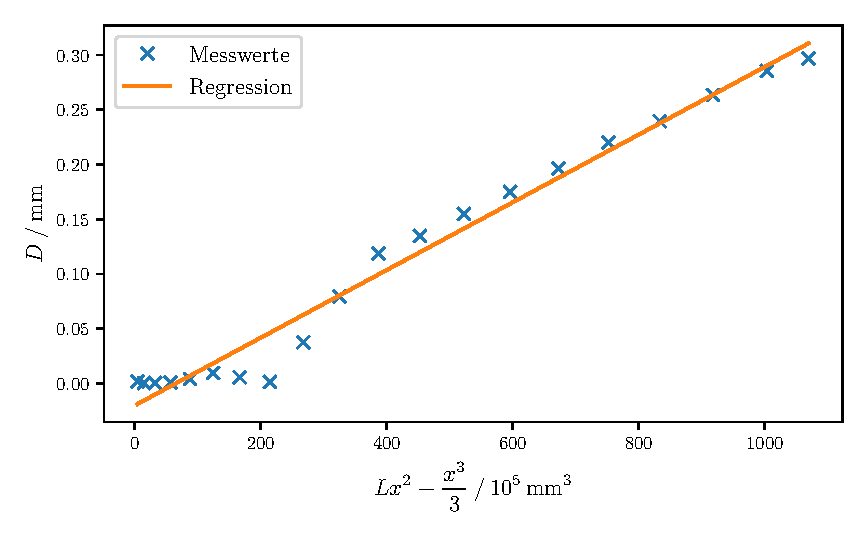
\includegraphics[scale=0.8]{build/plot_einseitig_eckig.pdf}
  \caption{Durchbiegung eines einseitig eingespannten eckigen Stabes, aufgetragen gegen einen Linearisierungsterm.}
  \label{fig:regression1}
\end{figure}

\subsection{Runder Stab, einseitig eingespannt} \label{sec:auswertung_einseitig_rund}
Zunächst wurde wieder eine Masse gewählt und fünfmal gewogen,
wobei sich im Mittel eine Masse von \SI{352.42 \pm 0.12}{\gram} ergab.

\begin{table}
\centering
\caption{Wiederholte Messung des benutzten Gewichts.}
\begin{tabular}{S}
\toprule
$m \mathbin{/} \si{\gram}$ \\
\midrule
352.2 \\
352.5 \\
352.4 \\
352.5 \\
352.5 \\
\bottomrule
\end{tabular}
\end{table}


In \autoref{tab:durchbiegung2} sind die Durchbiegung ohne Last ($D_\text{0}$), unter Last ($D_\text{M}$) und die tatsächliche Durchbiegung ($D$) mit der Position der Messuhr ($x$) aufgelistet.

\begin{table}
\centering
\caption{Durchbiegung des runden Stabes nach $x$-Abstand.}
\label{tab:durchbiegung2}
% \sisetup{table-format=2.1}
\begin{tabular}{c c c c}
\toprule
$x \mathbin{/} \si{\centi\meter}$ &
$D_0 \mathbin{/} \si{\micro\meter}$ &
$D_\text{M} \mathbin{/} \si{\micro\meter}$ &
$D \mathbin{/} \si{\micro\meter}$ \\
\midrule
\expandableinput{build/table_einseitig_rund.tex}
\bottomrule
\end{tabular}
\end{table}

\FloatBarrier

Es wurde $D(x)$ gegen den Linearisierungsterm $Lx^2-\frac{x^3}{3}$ aufgetragen (siehe \autoref{fig:regression2})
und mithilfe von NumPy eine Regressionsgerade $D(x) = k_2 \cdot x + c_2$ berechnet.
Deren Parameter sind:
\begin{align*}
  k_2 &= \SI{0.001454 \pm 0.000030}{\meter\tothe{-2}} \\
  c_2 &= \SI{-0.0027 \pm 0.0016}{\milli\meter} \; .
\end{align*}

Das Flächenträgheitsmoment $\mathbf{I}$ lässt sich diesmal durch \autoref{eqn:I_rund} mit den Abmessungen aus \autoref{sec:abmessungen} bestimmen.
%
% Die Gewichtskraft $F_G = g \cdot m$ ist durch die Erdbeschleunigung und die zuvor bestimmte Masse gegeben.

Schließlich ist
\begin{equation*}
  E
  = \frac{F_G}{2 k_2 \mathbf{I}}
  % Welch unintuitive Schreibweise! :/
  = \SI[{scientific-notation = true, separate-uncertainty = true}]{1.013(022)e5}{\newton\per\square\milli\meter}
\end{equation*}
der gesuchte Elastizitätsmodul.

% Die Messunsicherheit des Elastizitätsmoduls lässt sich gemäß der Gaußschen Fehlerfortpflanzung nach
% \begin{equation*}
%   \symup{\Delta}E = \frac{\partial E}{\partial m} \cdot \symup{\Delta}m
% \end{equation*}
% berechnen.

\begin{figure}
  \centering
  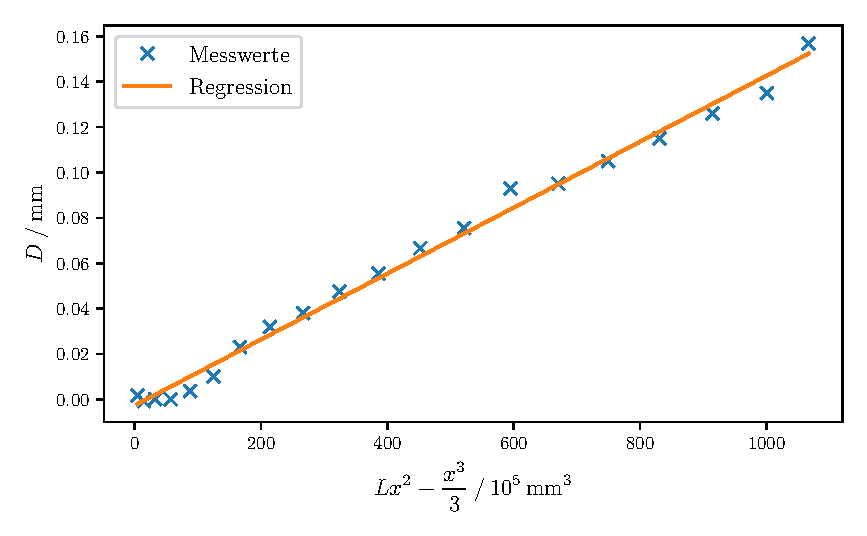
\includegraphics[scale=0.8]{build/plot_einseitig_rund.pdf}
  \caption{Durchbiegung eines einseitig eingespannten runden Stabes, aufgetragen gegen einen Linearisierungsterm.}
  \label{fig:regression2}
\end{figure}

\subsection{Runder Stab, beidseitig eingespannt} \label{sec:auswertung_beidseitig_rund}
Es wurde eine geeignete Masse gewählt und fünfmal gewogen,
wobei sich eine mittlere Masse von \SI{1005.980 \pm 0.074}{\gram} ergab.

\begin{table}
\centering
\caption{Wiederholte Messung des benutzten Gewichts.}
% \label{tab:todo}
% \sisetup{table-format=2.1}
\begin{tabular}{c}
\toprule
$m \mathbin{/} \si{\gram}$ \\
\midrule
\num{1005.9} \\
\num{1005.9} \\
\num{1006.0} \\
\num{1006.0} \\
\num{1006.1} \\
\bottomrule
\end{tabular}
\end{table}


In \autoref{tab:durchbiegung3} sind die Durchbiegung ohne Last ($D_\text{0}$), unter Last ($D_\text{M}$) und die tatsächliche Durchbiegung ($D$) mit der Position der Messuhr ($x$) aufgelistet.

\begin{table}
\centering
\caption{Durchbiegung des runden Stabes nach $x$-Abstand.}
\label{tab:durchbiegung3}
% \sisetup{table-format=2.1}
\begin{tabular}{c c c c}
\toprule
$x \mathbin{/} \si{\centi\meter}$ &
$D_0 \mathbin{/} \si{\micro\meter}$ &
$D_\text{M} \mathbin{/} \si{\micro\meter}$ &
$D \mathbin{/} \si{\micro\meter}$ \\
\midrule
\input{build/table_beidseitig_rund.tex}
\bottomrule
\end{tabular}
\end{table}

\FloatBarrier

Für die rechte Seite ($x \leq \frac{L}{2}$) wurde $D(x)$ gegen den Linearisierungsterm $3L^2x-4x^3$ aufgetragen (siehe \autoref{fig:regression3}), für die linke gegen $4x^3-12Lx^2+9L^2x-L^3$ (siehe \autoref{fig:regression4}).
Mithilfe von NumPy kann dann jeweils eine Regressionsgerade $D(x) = k_{3,4} \cdot x + c_{3,4}$ berechnet werden.
Deren Parameter sind
\begin{align*}
  k_3 &=
  \SI[{scientific-notation = true, separate-uncertainty = true}]
    {1.1(5)e-5}{\meter\tothe{-2}} \\
  c_3 &= \SI{-0.8 \pm 0.8}{\micro\meter}
\intertext{für die rechte und}
  k_4 &=
  \SI[{scientific-notation = true, separate-uncertainty = true}]
    {3.3(10)e-5}{\meter\tothe{-2}} \\
  c_4 &= \SI{-4.6 \pm 1.9}{\micro\meter}
\end{align*}
für die linke Seite.


Das Flächenträgheitsmoment $\mathbf{I}$ wird aus \autoref{sec:auswertung_einseitig_rund} übernommen.
%
% Die Gewichtskraft $F_G = g \cdot m$ ist durch die Erdbeschleunigung und die zuvor bestimmte Masse gegeben.

Schließlich sind
\begin{align*}
  E_\text{rechts}
  &= \frac{F_G}{2 k_3 \mathbf{I}}
  % Welch unintuitive Schreibweise! :/
  = \SI[{scientific-notation = true, separate-uncertainty = true}]{4.0(20)e7}{\newton\per\square\milli\meter} \\
  E_\text{links}
  &= \frac{F_G}{2 k_4 \mathbf{I}}
  % Welch unintuitive Schreibweise! :/
  = \SI[{scientific-notation = true, separate-uncertainty = true}]{1.3(04)e7}{\newton\per\square\milli\meter} \\
  \bar{E}
  % Welch unintuitive Schreibweise! :/
  &= \SI[{scientific-notation = true, separate-uncertainty = true}]{2.6(10)e7}{\newton\per\square\milli\meter}
  \tag{arithmetisches Mittel} \\
\end{align*}
die gesuchten Elastizitätsmoduln.

% Die Messunsicherheit des Elastizitätsmoduls lässt sich gemäß der Gaußschen Fehlerfortpflanzung nach
% \begin{equation*}
%   \symup{\Delta}E = \frac{\partial E}{\partial m} \cdot \symup{\Delta}m
% \end{equation*}
% berechnen.


\begin{figure}
  \centering
  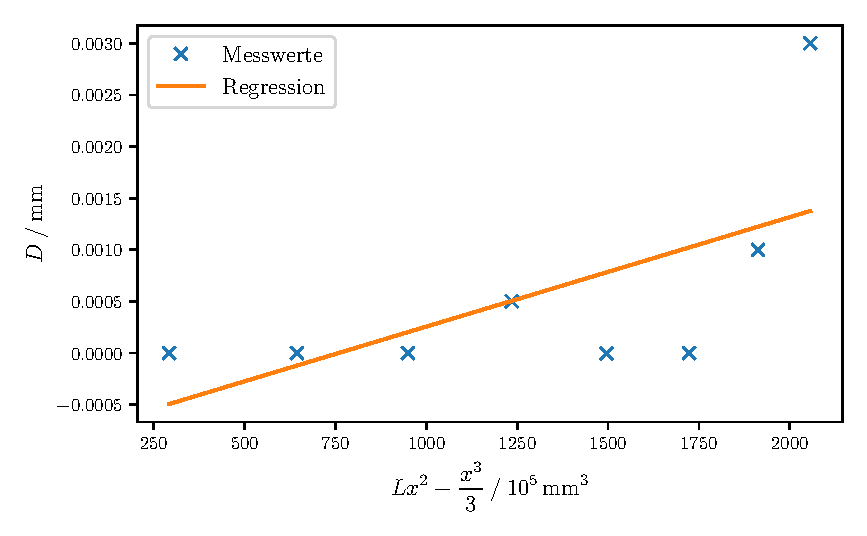
\includegraphics[scale=0.8]{build/plot_beidseitig_rund_rechts.pdf}
  \caption{Durchbiegung eines beidseitig eingespannten runden Stabes, aufgetragen gegen einen Linearisierungsterm: rechte Seite.}
  \label{fig:regression3}
\end{figure}

\begin{figure}
  \centering
  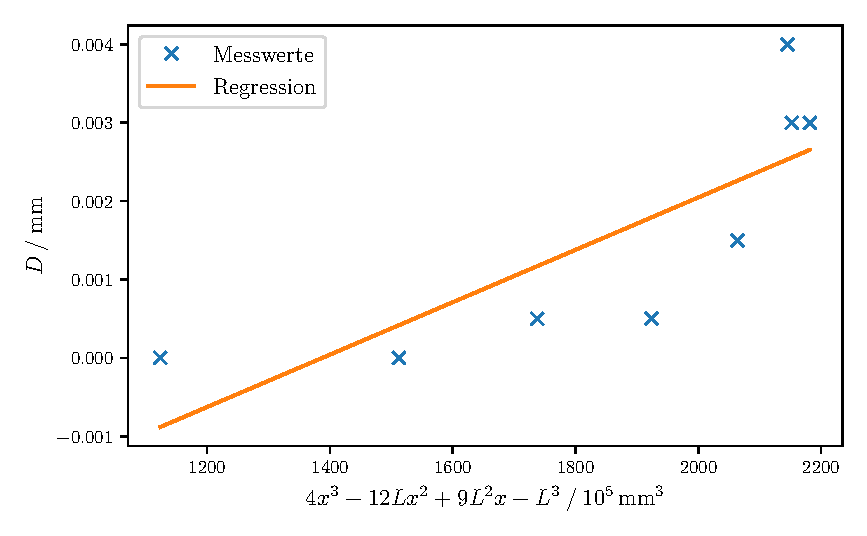
\includegraphics[scale=0.8]{build/plot_beidseitig_rund_links.pdf}
  \caption{Durchbiegung eines beidseitig eingespannten runden Stabes, aufgetragen gegen einen Linearisierungsterm: linke Seite.}
  \label{fig:regression4}
\end{figure}

